% \documentclass{article}

% % Language setting
% % Replace `english' with e.g. `spanish' to change the document language
% \usepackage[english]{babel}

% % Set page size and margins
% % Replace `letterpaper' with `a4paper' for UK/EU standard size
% \usepackage[letterpaper,top=2cm,bottom=2cm,left=3cm,right=3cm,marginparwidth=1.75cm]{geometry}

% % Useful packages
% \usepackage{amsmath}
% \usepackage{graphicx}
% \usepackage[colorlinks=true, allcolors=blue]{hyperref}

% \title{Your Paper}
% \author{You}

% \begin{document}
% \maketitle

% \begin{abstract}
% Your abstract.
% \end{abstract}

% \section{Introduction}

% Your introduction goes here! Simply start writing your document and use the Recompile button to view the updated PDF preview. Examples of commonly used commands and features are listed below, to help you get started.

% Once you're familiar with the editor, you can find various project settings in the Overleaf menu, accessed via the button in the very top left of the editor. To view tutorials, user guides, and further documentation, please visit our \href{https://www.overleaf.com/learn}{help library}, or head to our plans page to \href{https://www.overleaf.com/user/subscription/plans}{choose your plan}.

% \section{Some examples to get started}

% \subsection{How to create Sections and Subsections}

% Simply use the section and subsection commands, as in this example document! With Overleaf, all the formatting and numbering is handled automatically according to the template you've chosen. If you're using the Visual Editor, you can also create new section and subsections via the buttons in the editor toolbar.

% \subsection{How to include Figures}

% First you have to upload the image file from your computer using the upload link in the file-tree menu. Then use the includegraphics command to include it in your document. Use the figure environment and the caption command to add a number and a caption to your figure. See the code for Figure \ref{fig:frog} in this section for an example.

% Note that your figure will automatically be placed in the most appropriate place for it, given the surrounding text and taking into account other figures or tables that may be close by. You can find out more about adding images to your documents in this help article on \href{https://www.overleaf.com/learn/how-to/Including_images_on_Overleaf}{including images on Overleaf}.

% \begin{figure}
% \centering
% \includegraphics[width=0.25\linewidth]{frog.jpg}
% \caption{\label{fig:frog}This frog was uploaded via the file-tree menu.}
% \end{figure}

% \subsection{How to add Tables}

% Use the table and tabular environments for basic tables --- see Table~\ref{tab:widgets}, for example. For more information, please see this help article on \href{https://www.overleaf.com/learn/latex/tables}{tables}. 

% \begin{table}
% \centering
% \begin{tabular}{l|r}
% Item & Quantity \\\hline
% Widgets & 42 \\
% Gadgets & 13
% \end{tabular}
% \caption{\label{tab:widgets}An example table.}
% \end{table}

% \subsection{How to add Comments and Track Changes}

% Comments can be added to your project by highlighting some text and clicking ``Add comment'' in the top right of the editor pane. To view existing comments, click on the Review menu in the toolbar above. To reply to a comment, click on the Reply button in the lower right corner of the comment. You can close the Review pane by clicking its name on the toolbar when you're done reviewing for the time being.

% Track changes are available on all our \href{https://www.overleaf.com/user/subscription/plans}{premium plans}, and can be toggled on or off using the option at the top of the Review pane. Track changes allow you to keep track of every change made to the document, along with the person making the change. 

% \subsection{How to add Lists}

% You can make lists with automatic numbering \dots

% \begin{enumerate}
% \item Like this,
% \item and like this.
% \end{enumerate}
% \dots or bullet points \dots
% \begin{itemize}
% \item Like this,
% \item and like this.
% \end{itemize}

% \subsection{How to write Mathematics}

% \LaTeX{} is great at typesetting mathematics. Let $X_1, X_2, \ldots, X_n$ be a sequence of independent and identically distributed random variables with $\text{E}[X_i] = \mu$ and $\text{Var}[X_i] = \sigma^2 < \infty$, and let
% \[S_n = \frac{X_1 + X_2 + \cdots + X_n}{n}
%       = \frac{1}{n}\sum_{i}^{n} X_i\]
% denote their mean. Then as $n$ approaches infinity, the random variables $\sqrt{n}(S_n - \mu)$ converge in distribution to a normal $\mathcal{N}(0, \sigma^2)$.


% \subsection{How to change the margins and paper size}

% Usually the template you're using will have the page margins and paper size set correctly for that use-case. For example, if you're using a journal article template provided by the journal publisher, that template will be formatted according to their requirements. In these cases, it's best not to alter the margins directly.

% If however you're using a more general template, such as this one, and would like to alter the margins, a common way to do so is via the geometry package. You can find the geometry package loaded in the preamble at the top of this example file, and if you'd like to learn more about how to adjust the settings, please visit this help article on \href{https://www.overleaf.com/learn/latex/page_size_and_margins}{page size and margins}.

% \subsection{How to change the document language and spell check settings}

% Overleaf supports many different languages, including multiple different languages within one document. 

% To configure the document language, simply edit the option provided to the babel package in the preamble at the top of this example project. To learn more about the different options, please visit this help article on \href{https://www.overleaf.com/learn/latex/International_language_support}{international language support}.

% To change the spell check language, simply open the Overleaf menu at the top left of the editor window, scroll down to the spell check setting, and adjust accordingly.

% \subsection{How to add Citations and a References List}

% You can simply upload a \verb|.bib| file containing your BibTeX entries, created with a tool such as JabRef. You can then cite entries from it, like this: \cite{greenwade93}. Just remember to specify a bibliography style, as well as the filename of the \verb|.bib|. You can find a \href{https://www.overleaf.com/help/97-how-to-include-a-bibliography-using-bibtex}{video tutorial here} to learn more about BibTeX.

% If you have an \href{https://www.overleaf.com/user/subscription/plans}{upgraded account}, you can also import your Mendeley or Zotero library directly as a \verb|.bib| file, via the upload menu in the file-tree.

% \subsection{Good luck!}

% We hope you find Overleaf useful, and do take a look at our \href{https://www.overleaf.com/learn}{help library} for more tutorials and user guides! Please also let us know if you have any feedback using the Contact Us link at the bottom of the Overleaf menu --- or use the contact form at \url{https://www.overleaf.com/contact}.

% \bibliographystyle{alpha}
% \bibliography{sample}

% \end{document}


\documentclass[12pt,a4paper,oneside]{article}
\usepackage{amssymb}
\usepackage{amsmath}
\usepackage[pdftex]{graphicx,color}
\usepackage{cite}
\usepackage{graphicx}
\usepackage{amsmath,amsfonts}
\usepackage{longtable}
\usepackage{afterpage}
\usepackage{epstopdf}
\usepackage{amsthm}
\usepackage{booktabs} 
\usepackage{multirow}
\usepackage{float}
%\usepackage{caption}
%\usepackage{subcaption}
%\usepackage{url}
\thispagestyle{empty}
\usepackage{bbding}
\usepackage[margin=1in]{geometry} % Adjust margins as needed
\usepackage{array} % For table alignment


\renewcommand{\baselinestretch}{1.2}
\setlength{\textheight}{9.2in}
\setlength{\textwidth}{6.1in}
\addtolength{\leftmargin}{-.3in}
\topmargin -.2in
\pagenumbering{}

\begin{document}
	\pagestyle{empty}
	
	\begin{center}
\renewcommand{\baselinestretch}{1.8}

{\huge \bf A Data-Driven Fantasy Sports Analytics Platform}\\
\vspace{0.1 in}
{\huge \bf Cricsights}\\
\vspace{0.15 in}
{\small \bf A synopsis submitted\textcolor{white}{a}}\\
\vspace{0.15 in}
{\small \bf in Partial Fulfillment of the Requirements \textcolor{white}{a}}\\ 
\vspace{0.15 in}
{\small \bf for the Degree of\textcolor{white}{a}}\\ 
\vspace{0.15 in}
{\large \bf BACHELOR OF TECHNOLOGY\textcolor{white}{a}}\\ 
\vspace{0.15 in}
{\small \bf in\textcolor{white}{a}}\\ 
\vspace{0.15 in}
{\large \bf Department of Artificial Intelligence and Machine Learning\textcolor{white}{a}}\\ 
\vspace{0.15 in}
{\small \bf by\textcolor{white}{a}}\\ 
\vspace{0.15 in}
{\large \bf Srujan Kulkarni\textcolor{white}{a}}\\ 
\vspace{0.15 in}
{\large \bf Anand Gandhamwar\textcolor{white}{a}}\\ 
\vspace{0.15 in}
{\large \bf Avinash Parchake\textcolor{white}{a}}\\ 
\vspace{0.15 in}
{\small \bf Guided by\textcolor{white}{a}}\\ 
\vspace{0.15 in}
{\large \bf Swati Barik\textcolor{white}{a}}\\ 

\begin{figure}[!h]
\centering

\includegraphics[width=2.7in]{GHRCE_LOGO.png}
\end{figure}

{\Large \bf G H Raisoni College of Engineering and \textcolor{white}{a}}\\
\vspace{0.1 in}
{\Large \bf Management,\textcolor{white}{a}Wagholi, Pune} \\
\vspace{.2in}
{\large \bf (An Empowered Autonomous Institute  (Accredited by NAAC A$+$ Grade), Affiliated to SPPU, Pune} \\
\vspace{.2in}
{\small \bf January 2025}\\
\end{center}
 
	 
	\newpage
	\pagestyle{plain}
	\pagenumbering{arabic}
	
	\begin{center}
		{\huge \bf Synopsis}
	\end{center} 
\section{Abstract}
Cricsights is an advanced analytics platform designed to empower fantasy sports enthusiasts by providing real-time,
 pre-match, and post-match insights. Leveraging cutting-edge technologies such as machine learning and 
 data visualization, Cricsights delivers actionable insights through interactive and user-friendly interfaces.
  The platform offers comprehensive analytics, including player-specific, venue-specific, and matchup statistics, 
  enabling informed decision-making for fantasy cricket players. With features like real-time updates during matches 
  and meaningful visualizations, Cricsights bridges the gap between raw data and strategic decisions.
   The subscription-based model ensures accessibility for all users while catering to premium needs with live match analytics. 
   By transforming complex data into intuitive insights, Cricsights sets a new standard for fantasy sports engagement and decision-making.

    
\section{Introduction}

Crisights is a new platform designed to empower fantasy cricketers with data-driven tools to make smarter decisions.
 It offers comprehensive analytics, including real-time, pre- and post-match insights, with comprehensive statistics
  and an abundance of stunning graphics highlighting key elements such as players and play, location specific details,
   and on individual player performance, to enhance the CriSights gaming experience The platform provides tailored actionable 
   insights for its interactions It also builds user engagement through intuitive images, ensuring that users can quickly and 
   confidently make informed choices.
 \cite{greenwade93}.
% \section{Problem Statement}
% State the challenges faced by fantasy sports players, such as lack of real-time analytics and actionable insights.
% Discuss the gap Cricsights aims to fill in providing tailored, interactive data visualizations for decision-making.


\section{Objectives}
Objectives will come here.
\begin{enumerate}
	\item To design self-service analytical tools for fantasy players..
	
	\item To provide real-time, pre-match, and post-match insights.. 
	
    \item To empower users through meaningful data visualizations and interactive statistics..
\end{enumerate}

\section{Literature Review}
\subsection{Literature Survey Table}
The project draws from studies in computational literary analysis and network theory, 
\begin{longtable}{|c|p{4cm}|p{6cm}|p{5cm}|}
    \hline
    \textbf{Sr. No} & \textbf{Existing Tools} & \textbf{Identified Gaps} & \textbf{Cricsights Features} \\ \hline
    1 & ESPN Fantasy Sports
     & Minimal player-specific insights & Detailed individual player statistics \\ \hline
    2 & Generic Sports Websites  & Limited user interactivity and static visualizations & Interactive data exploration tools \\ \hline
    3 & Traditional Cricket Statistics Apps  & Lack of fantasy-relevant features & Insights tailored specifically for fantasy players \\ \hline
   
\end{longtable}
\subsection{Research Trends in Sports Analytics}
\begin{itemize}
    \item \textbf{Rise of Data-Driven Decision Making}:
    \begin{itemize}
        \item Adoption of data analytics in sports for performance optimization and strategy planning.
        \item Increasing reliance on predictive modeling for match outcomes and player performance.
    \end{itemize}
    \item \textbf{Machine Learning (ML) in Sports}:
    \begin{itemize}
        \item Use of ML algorithms for player performance prediction, injury risk assessment, and tactical analysis.
        \item Popular algorithms include regression models, decision trees, and neural networks.
    \end{itemize}
    \item \textbf{Data Visualization Tools}:
    \begin{itemize}
        \item Tools like Power BI and Tableau used for creating interactive dashboards and visual insights.
        \item Real-time visualizations help in understanding game dynamics and player statistics.
    \end{itemize}
\end{itemize}

\subsection{Comparison of Existing Solutions in Fantasy Sports}
\begin{itemize}
    \item \textbf{Current Solutions}:
    \begin{itemize}
        \item Platforms like Dream11 and FanDuel provide generic predictive insights based on basic statistics.
        \item Limited customization for user-specific decision-making.
        \item Lack of real-time updates and interactive analytics for live matches.
    \end{itemize}
    \item \textbf{Limitations}:
    \begin{itemize}
        \item Over-reliance on textual data and static reports.
        \item Inadequate visualization of complex data patterns.
        \item Minimal focus on venue-specific or player matchup statistics.
    \end{itemize}
\end{itemize}
\subsection{Architecture of Cricsights}
\begin{figure}[H]
    \centering
    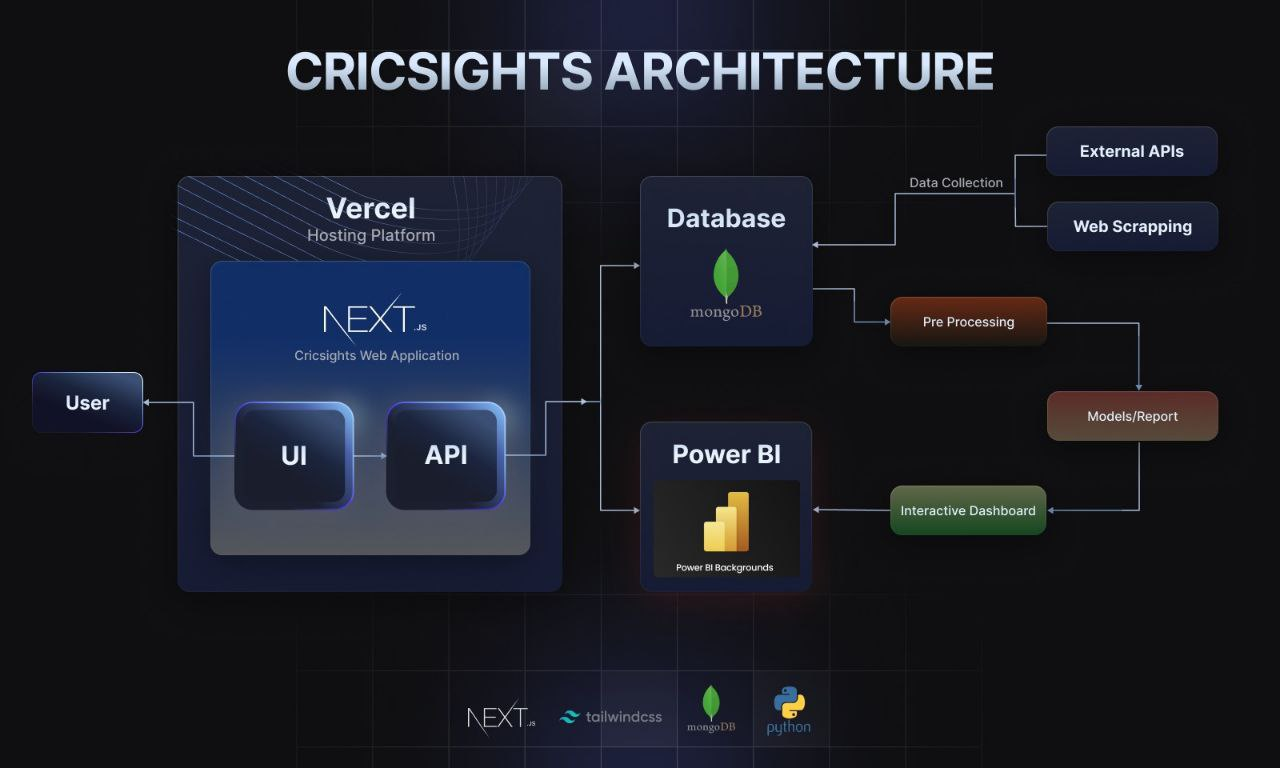
\includegraphics[width=\textwidth]{cricsight_architecuture.jpg}
    \caption{Cricsights System Architecture}
    \label{fig:architecture}
\end{figure}

% \section{Methodology}

% \subsection{Technology Stack}
% \begin{itemize}
%     \item \textbf{Frontend}:
%     \begin{itemize}
%         \item Next.js
%         \item React.js
%         \item Tailwind CSS
%     \end{itemize}
%     \item \textbf{Backend}:
%     \begin{itemize}
%         \item Node.js
%         \item Express.js
%     \end{itemize}
%     \item \textbf{Database}:
%     \begin{itemize}
%         \item MongoDB
%     \end{itemize}
%     \item \textbf{Analytics and Reporting}:
%     \begin{itemize}
%         \item Power BI
%     \end{itemize}
%     \item \textbf{Authentication and Authorization}:
%     \begin{itemize}
%         \item Firebase
%         \item OAuth
%     \end{itemize}
% \end{itemize}

% \subsection{Features to be Developed}
% \begin{itemize}
%     \item Real-time insights for live matches.
%     \item Pre-match and post-match analytics.
%     \item Player-specific and venue-specific statistics.
% \end{itemize}

% \subsection{Implementation Plan}
% The development and testing phases will be carried out step-by-step as follows:
% \begin{enumerate}
%     \item \textbf{Requirement Gathering}:
%     \begin{itemize}
%         \item Identify user needs and define the problem statement.
%         \item Analyze existing solutions and refine the scope.
%     \end{itemize}
%     \item \textbf{System Design}:
%     \begin{itemize}
%         \item Design the architecture for frontend, backend, and database.
%         \item Create mockups and prototypes for user interfaces.
%     \end{itemize}
%     \item \textbf{Development}:
%     \begin{itemize}
%         \item Develop the frontend using Next.js and Tailwind CSS.
%         \item Implement backend APIs using Node.js and Express.js.
%         \item Integrate MongoDB for data storage and retrieval.
%     \end{itemize}
%     \item \textbf{Integration and Testing}:
%     \begin{itemize}
%         \item Perform module-wise integration.
%         \item Conduct unit testing for individual modules and system testing for overall performance.
%     \end{itemize}
%     \item \textbf{Deployment and Maintenance}:
%     \begin{itemize}
%         \item Deploy the solution to a cloud platform for scalability and accessibility.
%         \item Monitor and maintain the platform for reliability and user satisfaction.
%     \end{itemize}
% \end{enumerate}
\section{Methodology}

\subsection{Data Collection}
\begin{itemize}
    \item \textbf{Sources:} Data is gathered from \textit{external APIs} and \textit{web scraping} techniques to ensure comprehensive coverage of player statistics, match details, and venue specifics.
    \item \textbf{Tools:} Python libraries like \texttt{requests} and \texttt{BeautifulSoup} are employed for scraping, while APIs are accessed through secure endpoints.
\end{itemize}

\subsection{Preprocessing}
\begin{itemize}
    \item The collected data undergoes cleaning and transformation to ensure consistency and usability.
    \item \textbf{Steps:}
    \begin{itemize}
        \item Handling missing or inconsistent data.
        \item Formatting data into structured formats suitable for database storage.
    \end{itemize}
    \item \textbf{Tools:} \texttt{Pandas} and \texttt{NumPy} in Python are utilized for data wrangling.
\end{itemize}

\subsection{Database Management}
\begin{itemize}
    \item \textbf{Database Used:} MongoDB is used to store the preprocessed data in a NoSQL format for scalability and quick querying.
    \item \textbf{Storage Structure:}
    \begin{itemize}
        \item Player-specific data.
        \item Match-specific analytics.
        \item Historical data for venue performance.
    \end{itemize}
\end{itemize}

\subsection{Analytics and Reporting}
\begin{itemize}
    \item \textbf{Dashboard Integration:} Power BI is employed for generating interactive dashboards, providing real-time insights and historical analytics for users.
    \item \textbf{Models and Reports:}
    \begin{itemize}
        \item Predictive analytics models are applied to deliver pre-match and post-match insights.
        \item Statistical reports for players and venues are generated.
    \end{itemize}
\end{itemize}

\subsection{Frontend Development}
\begin{itemize}
    \item \textbf{Framework:} Next.js and React.js are utilized to build a dynamic and responsive user interface (UI).
    \item \textbf{Styling:} Tailwind CSS is used to design an intuitive and user-friendly frontend for presenting analytics and dashboards.
    \item \textbf{Hosting:} Vercel is chosen for seamless hosting and deployment.
\end{itemize}

\subsection{Backend Development}
\begin{itemize}
    \item \textbf{Framework:} Node.js and Express.js are used for developing robust backend APIs.
    \item \textbf{API Functions:}
    \begin{itemize}
        \item Fetching real-time data for live match analysis.
        \item Serving pre-processed data for user dashboards.
    \end{itemize}
\end{itemize}

\subsection{Authentication}
\begin{itemize}
    \item \textbf{Methods:} Firebase and OAuth are implemented for secure and reliable user authentication.
    \item \textbf{Features:}
    \begin{itemize}
        \item User login and session management.
        \item Role-based access control for premium features.
    \end{itemize}
\end{itemize}

\subsection{User Interaction}
\begin{itemize}
    \item Users access the platform via a responsive web application, interacting with features such as:
    \begin{itemize}
        \item Real-time insights during live matches.
        \item Pre-match predictions and post-match analysis.
        \item Player and venue-specific statistics.
    \end{itemize}
\end{itemize}



\section{Project Plan and Timeline}

\begin{table}[h]
\begin{tabular}{|l|c|c|c|c|}
\hline
\multicolumn{1}{|c|}{\textbf{Activity/ Months}} & \textbf{Jan.'25} & \textbf{Feb.'25} & \textbf{Mar.'25} & \textbf{Apr.'25} \\ \hline
Problem Statement Identification                & \textbf{\checkmark}       & \textbf{}        & \textbf{}        & \textbf{}        \\ \hline
Literature Review                               & \textbf{\checkmark}       & \textbf{}        & \textbf{}        & \textbf{}        \\ \hline
Requirement Analysis                            & \textbf{\checkmark}       & \textbf{}        & \textbf{}        & \textbf{}        \\ \hline
Designing                                       & \textbf{}        & \textbf{\checkmark}       & \textbf{}        & \textbf{}        \\ \hline
Experimental Analysis                           & \textbf{}        & \textbf{\checkmark}       & \textbf{}        & \textbf{}        \\ \hline
Module-wise Implementation                      & \textbf{}        & \textbf{\checkmark}       & \textbf{\checkmark}       & \textbf{}        \\ \hline
Testing and Debugging                           & \textbf{}        & \textbf{}        & \textbf{\checkmark}       & \textbf{}        \\ \hline
Project Report Preparation                      & \textbf{}        & \textbf{}        & \textbf{}        & \textbf{\checkmark}       \\ \hline
\end{tabular}
\end{table}

\section{Expected Outcomes}
\begin{itemize}
    \item Development of an analytics platform tailored for fantasy sports enthusiasts.
    \item Enhanced user experience through interactive and meaningful insights.
    \item Real-time decision-making capabilities, empowering users during live matches.
\end{itemize}

\section{Business Model}
The revenue model for the platform includes free and premium services to cater to a wide range of users:
\begin{itemize}
    \item \textbf{Post-Match Analysis:} 
    \begin{itemize}
        \item This feature is free of charge and serves as an entry point to attract users to the platform.
    \end{itemize}
    \item \textbf{Pre-Match Analysis:}
    \begin{itemize}
        \item Available as a subscription-based service priced at \$x.
        \item Provides users with valuable insights and data to make informed decisions before a match.
    \end{itemize}
    \item \textbf{Live Match Analysis:}
    \begin{itemize}
        \item Offered as a premium feature priced at \$1.5x.
        \item Delivers real-time insights during cricket matches to enable dynamic and strategic decisions.
    \end{itemize}
\end{itemize}

	
		% \newpage
	
	%\addcontentsline{toc}{chapter}{Bibliography}
	
	
\bibliographystyle{IEEEtran}
\bibliography{sample}
Cricket analytics has been extensively explored in literature. For example, an analysis of the Indian Premier League (IPL) was carried out in \cite{ipl_analysis_prediction}. 
Similarly, machine learning methods have been applied for winning predictions in T20 cricket \cite{t20_prediction}.
Furthermore, player performance analysis using machine learning is discussed in \cite{player_performance_analysis}, 
and IPL data visualization techniques using Microsoft Power BI are presented in \cite{ipl_visualization}.




\vfill % Push the signing authority section to the bottom of the page

% Table for signing authorities
\begin{center}
\begin{tabular}{>{\centering\arraybackslash}m{0.3\textwidth}  % Column 1
                >{\centering\arraybackslash}m{0.3\textwidth}  % Column 2
                >{\centering\arraybackslash}m{0.3\textwidth}} % Column 3
    \textbf{Prof. Dhiraj Wyavahare} & \textbf{Dr. V. Y. Baviskar Dr. T. N. Mohota} & \textbf{Dr. R. Y. Sable} \\ 
    \textit{Project Guide} & \textit{Project Coordinator} & \textit{HoD, AI and AIML} \\
\end{tabular}
\end{center}

\end{document}